\documentclass[11pt]{article}
\usepackage{epsfig}
\usepackage{subfigure}
\usepackage{rotating} 
\usepackage{amsfonts,amssymb}
\usepackage{amsmath}
\usepackage{graphicx}
\usepackage[longnamesfirst,numbers]{natbib}
\usepackage{setspace}
\usepackage{pifont}
\usepackage{enumitem}
\usepackage{graphicx}
\usepackage{listings} %% mrb, see http://www.ctan.org/tex-archive/macros/latex/contrib/listings/

%\setlist{nolistsep,noitemsep,topsep=0pt,parsep=0pt,partopsep=0pt}
\setlist{nolistsep,itemsep=4pt,topsep=4pt,parsep=0pt,partopsep=0pt}
\DeclareGraphicsExtensions{.png,.jpg,.pdf}
\graphicspath{{./images/}}

\newcommand\commentout[1]{}
\newcommand\cvt{{\sc cvt}}

\def\Implies{\;\Longrightarrow\;}
\def\Equiv{\;\equiv\;}
\def\Equals{\;\;{\bf = }\;\;}
\def\And{\;\wedge\;}
\def\Or{\;\vee\;}

\headheight 0in
\parindent=0.0in
\parskip=2ex plus1ex
\topmargin 0.0in
\textheight 8.0in
\textwidth 6.250in
\evensidemargin -2.0mm
\oddsidemargin 4.0mm
%\evensidemargin 0.375in
%\oddsidemargin -0.03125in

\usepackage{fancyheadings}
\pagestyle{fancy}
\lhead{Independent Study}
\chead{}
\rhead{Cost Model Mining - Java Bytecode}
\lfoot{University of Colorado Boulder}
\cfoot{}
\rfoot{\ \thepage}

%\setcounter{page}{3}

\normalsize
\setlength{\headheight}{2\baselineskip}

\begin{document}

\vfill
\vfill

%\begin{center}
{\Large\bf{
Topic - Cost Model Mining in Java Bytecode}}


\vfill
\vfill
\vfill
\vfill

{\Large{Aniket Kumar Lata}}\newline
\\{\Large{Independent Study Report}}\newline
\\{\Large{Department of Electrical, Computer and Energy Engineering}}\newline
\\{\Large{University of Colorado Boulder}} \newline

\vfill
{\Large{Advised by:}}\newline
\\{\Large{Prof. Pavol {\v C}ern\'y }}\newline
\\{\Large{Dr. Ashutosh Trivedi}}\newline
\vfill
\vfill

July 22, 2016

\vfill
\vfill

\newpage
\tableofcontents
\newpage

\section{Introduction}
The cost model mining idea stemmed from the "Energy Disaggregation" concept . Energy disaggregation is the task of taking a whole-home energy signal and separating it into its component appliances. Our goal was to use the disaggregation idea and apply it to programs to fetch "execution time" of the different constituents of a program.\citep{energydisag}

Accurate execution time measurement of individual Java bytecode instructions is an important estimate in determining the total execution time of Java applications. There are a number of factors that make the execution time of Java bytecode difficult to predict. Java applications are run on a Java Virtual Machine (JVM) which translates Java bytecode to platform dependent machine code. It consists of stages that introduce optimizations in the translated machine code. A JIT compilation further introduces non determinism in the execution of a program. Dynamic linking and loading is another factor that slows down the compilation process of Java. C/C++ code is typically compiled to an object file then multiple object files are linked together to produce a usable artifact such as an executable or dll. During the linking phase symbolic references in each object file are replaced with an actual memory address relative to the final executable. In Java, this linking phase is performed dynamically at runtime. When a Java class is compiled, all references to variables and methods are stored in the class's constant pool as a symbolic reference.\citep{javabytecode} The JVM implementation can choose when to resolve symbolic references, this can happen when the class file is verified, after being loaded, called eager or static resolution, instead this can happen when the symbolic reference is used for the first time called lazy or late resolution.\citep{jvm} \newline

Due to these factors making Java programs less deterministic, it is useful to have a prediction mechanism that can provide a timing estimate for a block of instructions. My independent study builds upon this idea of timing blocks of code and predicting the execution time of applications that use these blocks. A cost model has been developed that can efficiently predict the execution time of basic blocks and methods declared within a program. Fetching costs for methods used in popular libraries can be a very useful measurement in profiling of Java programs.\newline

\textbf{What does the cost model do?}\newline
\\The cost model provides estimates pertaining to the execution time for expensive methods in Java bytecode. Java applications are profiled to generate: 
\begin{enumerate}
\item Counts of blocks/method invocations and 
\item Total execution time of the application  
\end{enumerate}
This profiling is performed with the help of bytecode instrumentation. The data generated from these runs is fed to a Linear Regression toolbox to efficiently predict the "time per basic block" or the "time per method" metric for that specific application.\newline

\textbf{What is its use?}\newline
\\The cost model tool can help in determining the time taken for each method or basic block to execute within an application. The worst case execution time (WCET) of a program is an important parameter which helps in real time scheduling applications. WCET can be predicted with the help of cost information from the model. The costs can be fed to a static analyses framework which can check all possible path combinations to get a WCET metric for that application. Cost modeling can also be used to detect security vulnerabilities in Java applications. Security vulnerabilities can be classified broadly into Availability and Confidentiality attacks. Availability problems arise when a user-provided input controls the asymptotic complexity or termination of a program component. The cost model can flag the blocks within a program that consume more CPU time with a high cost. A section of code susceptible to availability vulnerabilities can be determined by checking cost annotations of each block and what kind of inputs would reach this block of code.\newline

An important use of the cost model is to predict the execution time of Java applications whose libraries are profiled with the cost model. The model data forms a training input set and the application data forms a testing input set. The execution time of each method or basic block is an output from the training data set. These estimates are applied to the testing data set to predict the execution time of this application for a specific set of inputs.\newline

\textbf{Summary}\newline

The study involves developing a cost model tool which instruments Java bytecode to count bytecode instructions/blocks/methods being executed during an input run. The data generated from these executions is analysed using multiple linear regression. Cost model estimates are not always an accurate representation of the time being spent in the application. The regression algorithm may subsume some buckets over the other in cases of strong correlations between buckets. Also, there may be path imbalances within an application which may be detected only when the corresponding inputs are fed to the program. Hence, the estimates have a dependence on the "test inputs" and the "bucket refinement" being carried out by the cost model tool. Bucket refinement refers to the process of eliminating certain buckets depending on their correlation with existing buckets or their effect on the dependent variable which in this case is "execution time".

\newpage
\section{Motivating Examples and the Cost Model approach}
Java bytecode can be profiled at different points of interest to measure execution time for these sections of code. These measurements need to be consistent to ensure disambiguation of the timing analysis. To perform these measurements, we use instrumentation techniques for adding bytecode to existing applications. Bytecode instrumentation is a process where new functionality is added to a program by modifying the bytecode of a set of classes before they are loaded by the virtual machine. The JVM interprets that bytecode at runtime and then executes the correct native system instructions according to that bytecode.

\subsection{Basic Block Timing} 

We start our analysis by trying to disambiguate the execution time for basic blocks within a Java application. These are the most fundamental units of a program. Basic blocks present a straight-line code sequence making them highly amenable to analysis. These blocks have a singe entry point and a single exit point. Basic Blocks are useful in numerous program transformations and optimizations.\newline

Our aim in this section is to determine the time taken by basic blocks of a Java application to execute for a given set of inputs. One very straightforward approach in timing basic blocks is to identify the blocks and add timing code before and after the blocks. This analysis is termed as "Fine grain analysis". In the next subsection, we present experiments conducted with fine grain analysis, the results obtained and subsequent inferences.

\subsubsection{Fine grain analysis}
Java bytecode can be instrumented to add source code for timing the basic blocks within a program. We add System.nanotime() calls before and after each basic block and print the time measurement for each basic block. Our goal here is to verify if this method works accurately for execution time disambiguation of basic blocks. For disambiguation profiling, we consider an example program shown below with three basic blocks.\newline

\textbf{Examples}\newline
\begin{lstlisting}
public void workerFunction(int arg){
	int N = arg;
    int x = 0, a = 1, m = 0, i = 0;
    ArrayList<Integer> alist = new ArrayList<Integer>();

    if(N > 50) {
    		// Basic block 1 starts
        x++;
        x = x * N;
        x &= (a << 1);
        alist.add(x);
        // Basic block 1 ends
     }  else {
        		do{
               	// Basic block 2 starts
            		x += i;
                m = (x >> (N - i) & 1);
                i++;
                alist.add(x);
                // Basic block 2 ends
             }while(i < N);
        }
        if(x % 2 == 0) {
        		// Basic block 3 starts
            x = x * N;
            x %= N/3.14;
            x |= 34;
            java.lang.Thread.sleep(1);
            // Basic block 3 ends                   
        }
 }
\end{lstlisting}

The worker function is instrumented to measure execution time of the three basic blocks as shown in the modified worker function:

\singlespacing
\begin{lstlisting}
public void workerFunction(int arg){
	int N = arg;
    int x = 0, a = 1, m = 0, i = 0;
    ArrayList<Integer> alist = new ArrayList<Integer>();

    if(N > 50) {
    		// Basic block 1 starts
    		long l1 = System.nanoTime();
        x++;
        x = x * N;
        x &= (a << 1);
        alist.add(x);
        long l4 = System.nanoTime();
        long l7 = l4 - l1;
        double d = (double)l7 / 1000000D;
        System.out.println((new StringBuilder()).append("\n\rDURATION: 
        ").append(d).toString());
        // Basic block 1 ends
     }  else {
        		do{
               	// Basic block 2 starts
				long l2 = System.nanoTime();               	
            		x += i;
                m = (x >> (N - i) & 1);
                i++;
                alist.add(x);
                long l6 = System.nanoTime();
                long l9 = l6 - l2;
                double d2 = (double)l9 / 1000000D;
                System.out.println((new StringBuilder()).append(
                "\n\rDURATION: ").append(d2).toString());
                // Basic block 2 ends
             }while(i < N);
        }
        if(x % 2 == 0) {
        		// Basic block 3 starts
        		long l3 = System.nanoTime();
            x = x * N;
            x %= N/3.14;
            x |= 34;
            java.lang.Thread.sleep(1);
            long l5 = System.nanoTime();
            long l8 = l5 - l3;
            double d1 = (double)l8 / 1000000D;
            System.out.println((new StringBuilder()).append(
            "\n\rDURATION: ").append(d1).toString());
            // Basic block 3 ends                   
        }
 }
\end{lstlisting}
\newpage

\textbf{Results}\newline

The basic block measurements were tested by executing the instrumented version of the code multiple times with the same input.\newline

\textbf{Commands:} \\
\$ java -jar Test.jar 8\\
\$ java -jar Test.jar 56\\	  

\textbf{Run 1:}

Execution time measurements in milliseconds(ms):\\
\\Basic block 1: 0.440963 \\
\\Basic block 2:\\
\hspace{2em} Iteration 1: 0.332355\\
\hspace{2em} Iteration 2: 0.0012\\
\hspace{2em} Iteration 3: 0.001012\\
\hspace{2em} Iteration 4: 0.000965\\
\hspace{2em} Iteration 5: 0.000966\\
\hspace{2em} Iteration 6: 0.000887\\
\hspace{2em} Iteration 7: 0.000926\\
\hspace{2em} Iteration 8: 0.000914\\
\\Basic block 3: 1.11022\\

\textbf{Run 2:}

Execution time measurements in milliseconds(ms):\\
\\Basic block 1: 0.318824\\
\\Basic block 2:\\
\hspace{2em} Iteration 1: 0.310898\\
\hspace{2em} Iteration 2: 0.001169\\
\hspace{2em} Iteration 3: 0.001046\\
\hspace{2em} Iteration 4: 0.000961\\
\hspace{2em} Iteration 5: 0.000945\\
\hspace{2em} Iteration 6: 0.000895\\
\hspace{2em} Iteration 7: 0.000904\\
\hspace{2em} Iteration 8: 0.000867\\
\\Basic block 3: 1.086663\\

\textbf{Run 3:}

Execution time measurements in milliseconds(ms):\\
\\Basic block 1: 0.299579\\
\\Basic block 2:\\
\hspace{2em} Iteration 1: 0.373075\\
\hspace{2em} Iteration 2: 0.001417\\
\hspace{2em} Iteration 3: 0.001294\\
\hspace{2em} Iteration 4: 0.00115\\
\hspace{2em} Iteration 5: 0.001131\\
\hspace{2em} Iteration 6: 0.001112\\
\hspace{2em} Iteration 7: 0.001073\\
\hspace{2em} Iteration 8: 0.001084\\
\\Basic block 3: 1.089375\\

\textbf{Run 4:}

Execution time measurements in milliseconds(ms):\\
\\Basic block 1: 0.310518\\
\\Basic block 2:\\
\hspace{2em} Iteration 1: 0.317869\\
\hspace{2em} Iteration 2: 0.001171\\
\hspace{2em} Iteration 3: 0.001075\\
\hspace{2em} Iteration 4: 0.000916\\
\hspace{2em} Iteration 5: 0.001008\\
\hspace{2em} Iteration 6: 0.000965\\
\hspace{2em} Iteration 7: 0.000921\\
\hspace{2em} Iteration 8: 0.000934\\
\\Basic block 3: 1.095043

\textbf{Statistics: }\\

\begin{center}
\begin{tabular}{|c|c|c|c|}
\hline
Blocks&Mean&Standard Deviation&Variance\\
\hline
Basic block 1&0.34247&0.06613&0.00437\\
Basic block 2&0.34247&0.06613&0.00437\\
Basic block 3&1.09533&0.01053&0.00011\\
\hline
\end{tabular}
\end{center}

\textbf{Inference}\newline
\\Disambiguation among the execution time measurements can be ensured if the timing measurements are consistent. From the above measurements, it can be seen that the variance is significant considering the fact that timing measurements require very high accuracy. Basic block 2 has a large standard deviation from the mean taking into account all the four runs of this application. It should be noted that the input argument was the same for each run. Basic block 1 is reachable with inputs greater than 50 and basic block 2 is reachable when input argument is less than 50. The statistics show that even though the inputs did not vary, there is significant amount of variance in the timings.

\subsubsection{Disambiguation}
The fine grain approach does not work in disambiguation of execution time for basic blocks as the standard deviation of the reading is significant when multiple runs are accounted. We propose a novel approach to disambiguate execution time for Java applications. The cost model profiles a program to measure the execution time for one entire run as opposed to timing individual sections of code. Instrumentation is added to fetch block invocation counts.  \newline
The basic example would be profiled as shown in the subsequent sections to generate a cost model.

\textbf{Execution time Profiling}
\begin{lstlisting}
public void workerFunction(int arg){
	// Instrumentation for exec time 
	long startTime = System.nanoTime();
	int N = arg;
    int x = 0, a = 1, m = 0, i = 0;
    ArrayList<Integer> alist = new ArrayList<Integer>();

    if(N > 50) {
    		// Basic block 1 starts
        x++;
        x = x * N;
        x &= (a << 1);
        alist.add(x);
        // Basic block 1 ends
     }  else {
        		do{
               	// Basic block 2 starts
            		x += i;
                m = (x >> (N - i) & 1);
                i++;
                alist.add(x);
                // Basic block 2 ends
             }while(i < N);
        }
        if(x % 2 == 0) {
        		// Basic block 3 starts
            x = x * N;
            x %= N/3.14;
            x |= 34;
            java.lang.Thread.sleep(1);
            // Basic block 3 ends                   
        }
      long endTime = System.nanoTime();
      long elapsedTime = endTime - startTime;
      double duration = (double)elapsedTime / 1000000.0;
      System.out.println(duration);
 }
\end{lstlisting}

\textbf{Block invocation Profiling}
\begin{lstlisting}
public void workerFunction(int arg){
	// Instrumentation for block invocation counts
	// counters: counter_bb1, counter_bb2, counter_bb3
	int counter_bb1 = 0, counter_bb2 = 0, counter_bb3 = 0;
	int N = arg;
    int x = 0, a = 1, m = 0, i = 0;
    ArrayList<Integer> alist = new ArrayList<Integer>();

    if(N > 50) {
    		// Basic block 1 starts
        x++;
        x = x * N;
        x &= (a << 1);
        alist.add(x);
        counter_bb1++;
        // Basic block 1 ends
     }  else {
        		do{
               	// Basic block 2 starts
            		x += i;
                m = (x >> (N - i) & 1);
                i++;
                alist.add(x);
                counter_bb2++;
                // Basic block 2 ends
             }while(i < N);
        }
        if(x % 2 == 0) {
        		// Basic block 3 starts
            x = x * N;
            x %= N/3.14;
            x |= 34;
            counter_bb3++;
            java.lang.Thread.sleep(1);
            // Basic block 3 ends                   
        }
 }
\end{lstlisting}


Model generation requires two passes for each input: execution time pass and block invocation count pass. This data is logged on the disk for a large number of inputs.\newline 

\textbf{Results}

The cost model disambiguation approach was tested on the same basic blocks example. The inputs to the application were randomly generated. Below are the results obtained:

Output 1: Number of runs consists of 800 distinct inputs

Coefficients:

workerFunction\_basicBlock1: 0.2212857\\
workerFunction\_basicBlock2: 0.0095599\\
workerFunction\_basicBlock3: 1.2227574\\

Output 2: Number of runs consists of 1600 distinct inputs

Coefficients:

workerFunction\_basicBlock1: 0.2438942\\
workerFunction\_basicBlock2: 0.0096788\\
workerFunction\_basicBlock3: 1.2122846\\


Output 3: Number of runs consists of 2400 distinct inputs

Coefficients:

workerFunction\_basicBlock1: 0.2099943\\
workerFunction\_basicBlock2: 0.0088905\\
workerFunction\_basicBlock3: 1.2196536\\

Output 4: Number of runs consists of 3200 distinct inputs

Coefficients:

workerFunction\_basicBlock1: 0.2156011\\
workerFunction\_basicBlock2: 0.0089118\\
workerFunction\_basicBlock3: 1.2254903\\


\textbf{Statistics: }

\begin{center}
\begin{tabular}{|c|c|c|c|}
\hline
Blocks&Mean&Standard Deviation&Variance\\
\hline
Basic block 1&0.22269&0.01487&0.00022\\
Basic block 2&0.00926&0.00042&0\\
Basic block 3&1.22005&0.0057&0.00003\\
\hline
\end{tabular}
\end{center}


\textbf{Inference}

The cost model disambiguation approach shows that there is minimal standard deviation for each basic block timing estimate, much lower than the fine grain analysis approach. As it can be seen, the variance is 0 for basic block 2 whereas the fine grain approach showed much higher variance for this basic block.
\newpage

\subsection{Bytecode Instruction disambiguation}
A very straightforward approach to determine execution time of a set of bytecode instructions is to place a timer before and after these instructions. Our initial analysis will revolve around this idea where we target a piece of source code and try to determine the time that this piece of code takes to execute on the given platform. Here, we are trying to establish that at which level do we can we achieve disambiguation using this fine grain approach. 

\subsubsection{Fine grain analysis}

The program given below demonstrates timing the arithmetic instructions one at a time and printing the output. We analyse to check if we get a consistent timing for each of these instructions on the instruction granularity level.

\begin{lstlisting}
public class FineGrainTiming {
        public static void main(String[] args) {
                int a = Integer.parseInt(args[0]);
                int b = Integer.parseInt(args[1]);
                long lStartTime = System.nanoTime();
                int c = a + b;
                long lEndTime = System.nanoTime();
                long difference = lEndTime - lStartTime;
                System.out.println("Add: " + difference);
                lStartTime = System.nanoTime();
                int d = a - b;
                lEndTime = System.nanoTime();
                difference = lEndTime - lStartTime;
                System.out.println("Sub: " + difference);
                lStartTime = System.nanoTime();
                int e = a * b;
                lEndTime = System.nanoTime();
                difference = lEndTime - lStartTime;
                System.out.println("Mul: " + difference);
                lStartTime = System.nanoTime();
                int f = a / b;
                lEndTime = System.nanoTime();
                difference = lEndTime - lStartTime;
                System.out.println("Div: " + difference);
        }
}
\end{lstlisting}

The results of the granular timing are compared with overall execution time of the application obtained by executing the following program.

\singlespacing
\begin{lstlisting}
public class GetExecutionTime {
        public static void main(String[] args) {
                int a = Integer.parseInt(args[0]);
                int b = Integer.parseInt(args[1]);
                long lStartTime = System.nanoTime();
                int c = a + b;
                int d = a - b;
                int e = a * b;
                int f = a / b;
                long lEndTime = System.nanoTime();
                long difference = lEndTime - lStartTime;
                System.out.println("Time: " + difference);
        }
}
\end{lstlisting}

\textbf{Results:}

Both these programs are executed with the same inputs for comparison. Let's consider case 1: 

\$ java BinTime 97989 8007

Execution 1: \\
Add: 149\\
Sub: 233\\
Mul: 173\\
Div: 198\\
\\Execution 2:\\
Add: 150\\
Sub: 167\\
Mul: 92\\
Div: 125\\
\\Execution 3:\\
Add: 140\\
Sub: 165\\
Mul: 158\\
Div: 185\\
\\\\Execution 4:\\
Add: 187\\
Sub: 327\\
Mul: 259\\
Div: 293\\
\\Execution 5:\\
Add: 137\\
Sub: 158\\
Mul: 161\\
Div: 151\\

Below are the results of execution time of the program which is considered as case 2:

Execution 1: 206\\
Execution 2: 357\\
Execution 3: 199\\
Execution 4: 191\\
Execution 5: 216\\

\textbf{Inference}

On comparing the fine grain timing with the execution time of entire application for a Java program, it can be seen the the granular timing introduces a very high amount of overhead into the timing. This results in high amount of error and it does not match the overall execution time measurement. Thus, we see that we need a different method to disambiguate the execution time on the instruction level. One such approach is presented in the next section.\\

\subsubsection{Cost Model approach}

The cost model approach can be applied at the bytecode level to disambiguate different types of bytecode instructions and their execution times on a target platform. In this example, the disambiguation of bytecode instructions has been performed for an arithmetic intensive program.

\begin{lstlisting}
public class TestBinaryOp {
        public static void main(String[] args) {
                int x = Integer.parseInt(args[0]);
                int y = Integer.parseInt(args[1]);
                int numAdd = Integer.parseInt(args[2]);
                int numSub = Integer.parseInt(args[3]);
                int numMul = Integer.parseInt(args[4]);
                int numDiv = Integer.parseInt(args[5]);
                int result;
              
                for( int i = 0; i < numAdd; i++ ) {
                        result = x + y;
                }
                for( int i = 0; i < numSub; i++ ) {
                        result = x - y;
                }
                for( int i = 0; i < numMul; i++ ) {
                        result = x * y;
                }
                for( int i = 0; i < numDiv; i++ ) {
                        result = x / y;
                }
        }
}
\end{lstlisting}

The bytecode instructions have been divided into the following categories for disambiguation.
\begin{lstlisting}
ADD           - ADD
SUBTRACT      - SUB
MULTIPLY      - MUL
DIVIDE        - DIV
CALLS         - Method Calls
LDSTCOND      - LOAD,STORE,PUSH,POP,GETSTATIC,CONST,IFEQ,GOTO,ICMP,INC,I2D
\end{lstlisting}

Below are the estimates for the bytecode instructions:\\
\begin{center}
\begin{tabular}{|c|c|}
\hline
Instruction&Estimate\\
\hline
ADD&7.139393e-06\\
SUBTRACT&7.476836e-06\\
MULTIPLY&6.896982e-06\\
DIVIDE&9.236163e-06\\
CALLS&0.006411416\\
\hline
\end{tabular}
\end{center}

We have estimates for add, subtract, multiply and divide bytecode instructions. Let us now test the accuracy of these estimates with the help of a simple program making use of arithmetic instructions only.\newline

\singlespacing
\begin{lstlisting}
public class TestArithmeticOperations {
        public static void main(String[] args) {
                int a = Integer.parseInt(args[0]);
                int b = Integer.parseInt(args[1]);
                for(int i = 0; i < 2000; i++){
                        int c = a + b;
                        int d = a - b;
                        int e = a * b;
                        int f = a / b;
                }
        }
}
\end{lstlisting}

We have instrumented the above example program to measure execution time of the entire program for a set of inputs. Another form of instrumentation measures the bytecode counts for ADD, SUBTRACT, MULTIPLY, DIVIDE operations and the function calls within the program. We will be applying the estimates generated by our model to predict the execution time of this application. The predicted time will be compared to the actual execution time measured earlier.\newline

\begin{equation}
Predicted Time = \sum_{i} estimate_{i} * count_{i}  
\end{equation}
\vspace{0.5em}
where i $\epsilon$ \{bytecode instructions\}

On substituting the estimates obtained, we get,\\
\textbf{Predicted Time} = 0.07424ms

Actual time is considered here as a mean of 15 executions of the program
\textbf{Actual time} = 0.07612ms\\

As we can see here, the difference between predicted time and actual time is not much. With this experiment, we make a proposition that each of the bytecode instructions can be disambiguated using the cost model approach and the estimates can be applied in real life applications to predict execution time of these applications.

It can be seen here that the cost for arithmetic instructions: Add, Subtract, Multiply, Divide has been estimated by the model. However, at the lowest level this disambiguation can tend to have some deviation depending on the interference from other instructions to the measurement of arithmetic and related bytecode costs.\newline
\newpage

\subsection{Method disambiguation}
We have seen that timing basic blocks for the same input produces inconsistent results. Our approach relies on timing the entire application as opposed to timing each fundamental unit of the program. With the cost model, we measure the execution time of the application and log method invocation counts for a number of inputs. Linear regression is used to produce the estimates for each method. The example given below illustrates our approach.

\singlespacing
\begin{lstlisting}
public class Functions {
	
	public void function1() throws InterruptedException{
		java.lang.Thread.sleep(1);
	}
	
	public void function2() throws InterruptedException{
		java.lang.Thread.sleep(10);
	}
	
	public void function3() throws InterruptedException{
		java.lang.Thread.sleep(500);
	}
	
	public void function4() throws InterruptedException{
		java.lang.Thread.sleep(100);
	}
	
	public void function5(){
		return;
	}
	
}
\end{lstlisting}

The "Functions" library consists of five functions and each one takes different amounts of time to execute. Our goal here is to disambiguate these functions by accurately identifying the amount of time for which they run. \newline

The cost model approach instruments the Functions library to fetch method invocation counts and total execution time for the application. The cost model is explained in detail in the later sections. A test application has been written that calls the methods in the library with different call distributions. As it can be seen in the test class below, methods are invoked in different order for different inputs received from the users. This exercise simulates a good coverage of the functions being called in random distributions.

\subsubsection{Basic example}
\begin{lstlisting}
public class MainFunc {
	
	public static void main(String args[]) throws InterruptedException{
		
		int N = Integer.parseInt(args[0]);
		Functions func = new Functions();
		
		switch(N){
			case 1:
				func.function1();
				func.function3();
				func.function3();
				func.function5();
				func.function3();
				break;
			case 2:
				func.function5();
				func.function2();
				func.function2();
				func.function4();
				func.function4();
				break;
			case 3:
				func.function3();
				func.function4();
				func.function4();
				func.function5();
				func.function4();
				break;
			case 4:
				func.function1();
				func.function1();
				func.function5();
				func.function4();
				func.function2();
				break;
			case 5:
				func.function1();
				func.function1();
				func.function1();
				func.function2();
				func.function1();
				break;
			case 6:
				func.function5();
				func.function4();
				func.function3();
				func.function2();
				func.function1();
				break;
			}
		}		
}
\end{lstlisting}

\textbf{Initial Results}

Multiple linear regression is used to generate the best fitting estimates that can disambiguate the time taken by each method. The dependent variable is "execution time" for a specific run and the independent variables are "method names" for that same run. The estimates are generated for each independent variable which are the "functions" in the above example. The estimates generated using our cost model tool for 200 inputs are as shown below: \newline

\begin{center}
\begin{tabular}{|c|c|}
\hline
Function&Estimate\\
\hline
Function1&1.131e+00  \\
Function2&1.014e+01  \\
Function3&5.002e+02  \\
Function4&1.002e+02  \\
Function5&2.807e-02  \\
\hline
\end{tabular}
\end{center}

As it can be seen, the estimates generated are quite accurate. We can compare the estimates to the sleep call parameters within each function as the functions are not doing any other work. These estimates become more and more precise as the input coverage gets better and the number of test inputs increases. \newline

Thus, it can be inferred from this experiment that the method disambiguation experiment worked well using the cost model for the basic example illustrated. 

\subsubsection{Problems with method disambiguation}
Method disambiguation worked well in the example demonstrated in section 2.2.1. The methods used in the library did not have any control flows. If the method is a sequential block of statements, for a single input the same section of code will be executed. However with control flows being a part of the method, different branches are executed for differing inputs to the program. This can be illustrated well by modifying the basic example presented earlier.\newline

Control flows introduce path imbalances in the program execution. In such cases, it becomes difficult to provide an estimate for the execution time of such methods if the  execution time of paths taken for an input is noticeably different.

\subsubsection{Control flow example}
\begin{lstlisting}
public void function1() throws InterruptedException{
	java.lang.Thread.sleep(20);
}
	
public void function2(int n) throws InterruptedException{
	java.lang.Thread.sleep(5);
	if(n > 6)
		function4();	
}
	
public void function3() throws InterruptedException{
	java.lang.Thread.sleep(500);
}
	
public void function4() throws InterruptedException{	
	java.lang.Thread.sleep(100);
}
	
public void function5(){
	return;
}
\end{lstlisting}

\textbf{Results}

The control flow example in section 2.3.1 is a modification of the basic example shown with methods. We have a branch in function2() which changes the predicted estimates significantly. It can be seen that function5() gets a negative estimate and the estimate for function4() is incorrect. function2() has a branch and it's estimate will vary depending upon the value of 'n'. It is incorrect to have an estimate for functions where the control flow determines the execution time of the program.\newline

\begin{center}
\begin{tabular}{|c|c|}
\hline
Function&Estimate\\
\hline
function1&21.323\\
function2&39.599\\
function3&500.569\\
function4&5.361\\
function5&-0.907\\
\hline
\end{tabular}
\end{center}

The aim of this example was to illustrate the amount of inaccuracy that a branch can introduce within the cost measurements. Real life programs will have a large number of branches and if these branches introduce paths that are significantly different from one another in terms of execution time, it is necessary to mitigate the effects of control flows within a program. \newline
\newpage

\subsection{Cost Model}
We have tested the cost model approach on instruction, basic block and method level. It could be seen that on the instruction and method level, the standard error with our estimates is high due to the presence of correlation between our independent variables in regression. In the following example, we highlight the problem of correlation between buckets.

\subsubsection{Correlation}

Let us have a look at the following Modular exponentiation class. It consists of three basic blocks.

\singlespacing
\begin{lstlisting}
public class ModularExponentiation {
	public static void main(String args[]) throws InterruptedException {
    		Integer x = Integer.parseInt(args[0]);
        Integer e = Integer.parseInt(args[1]);
        Integer N = Integer.parseInt(args[2]);
		squareMult(x, e, N);
   	}

	public static Integer squareMult(Integer x, Integer e, Integer N) 
	throws InterruptedException{
    		ArrayList<Integer> alist = new ArrayList<Integer>();
        Integer y = 1;
        int n = Integer.SIZE;
        int i = n;
        do {
        			// basic block 1 starts
            		y = y * y;
                y = y % N;
                //basic block 1 ends
                if(((e >> (n-i)) & 1) == 1){
                		// basic block 2 starts
                		y = y * x;
                    java.lang.Thread.sleep(10);
                    y = y % N;
                    // basic block 2 ends
                }
                // basic block 3 starts
                i--;
                alist.add(y);
                // basic block 3 ends
           } while(i >= 1);
    		return y;
    }
}
\end{lstlisting}

On running our cost model over this program for 800 distinct inputs, we get the below estimates for basic blocks 1,2 and 3.\\

Coefficients:\\
Basic block 1: 0.01217091\\
Basic block 2: 10.10931665\\
Basic block 3: NA\\

It can be clearly seen that basic blocks 1 (bb1) and 3 (bb3) are executed each time and hence the block invocation count for these blocks will be 1 for all the executions. The execution of basic block 2 is dependent on a condition. It can be said that there is a high correlation between basic blocks 1 and 3 such that every time bb1 is executed, bb3 is also executed and vice versa. Our cost model is unable to disambiguate between basic blocks 1 and 3 from the statistics that we obtain after profiling. The profiling procedure is explained in detail in the Implementation section. The estimate obtained for bb1 is actually the estimate for bb1 and bb3 combined. The linear regression algorithm accounts for only one of these two independent variables and generates an estimate for this variable.\newline 

In the next section, we will present some techniques that can help refine the cost model by reducing the effect of correlation and thus, the standard error for each estimate.
\newpage

\section{Cost Estimation}
\subsection{Multiple Linear Regression}
Our cost model needs to predict the value of the dependent variable -- execution time, using a linear function of the independent variables -- method counts.

A naive approach to bucketing would be accounting for each method used in the application as a separate bucket. The standard error for coefficients in multiple regression can be high if we don't account for the correct subsets of independent variables in the model. The variance of coefficient for a variable could increase if there is high correlation among with another variable. The mean squared error for all the variables gives a good indication of the estimate provided by the cost model. Even though a model shows an ideal coefficient of determination, it may not be sufficient to give an accurate estimate for an independent test application using the same independent variables i.e. methods in our case. There is a need to refine the cost model to address the standard error among variables within a model and the mean squared error for accurate estimation of test applications.\newline
\\\textbf{Subset Selection}

An important decision to be made is the bucketing (categorization) of methods in a Java application to perform multiple linear regression. This is termed as ``subset selection'' for the model. The naive approach considers all independent variables in the data for prediction. There are several reasons why this could be undesirable:
\begin{itemize}
\item Estimates of regression coefficients are likely to be unstable due to multi-collinearity in models with many variables. 
\item We get better insights into the influence of regressors from models with fewer variables as the coefficients are more stable for parsimonious models.
\item It can be shown that using independent variables that are uncorrelated with the dependent variable will increase the variance of predictions.
\item It can be shown that dropping independent variables that have small (non-zero) coefficients can reduce the average error of predictions.
\end{itemize}

\begin{equation}
Y = \beta_{0} + \beta_{1}X_{1}+ \beta_{2}X_{2} + \dotsb+ \beta_{n}X_{n}
\end{equation}
\vspace{0.5em}
\begin{equation}
MSE = \frac{1}{N} \sum_{i=0}^{N} (y_{i} - \hat{y_{i}})^{2}
\end{equation}

\textbf{Multicollinearity}

In regression, "multicollinearity" refers to predictors that are correlated with other predictors.  Multicollinearity occurs when your model includes multiple factors that are correlated not just to your response variable, but also to each other.\citep{linearreg} In other words, it results when you have factors that are a bit redundant.
Multicollinearity increases the standard errors of the coefficients. Increased standard errors in turn means that coefficients for some independent variables may be found not to be significantly different from 0. In other words, by overinflating the standard errors, multicollinearity makes some variables statistically insignificant when they should be significant. \newline
\\The problem of multicollinearity can be addressed by removing buckets that have high correlation with one of the other buckets in the data. If two buckets are correlated, only one of the buckets should be considered. All the buckets that are processed should have negative correlation or a very small positive correlation. Below is an R script which filters the data for multicollinearity. 


\begin{lstlisting}
args <- commandArgs(TRUE)
x = read.csv(args[1], header=TRUE)
a = as.matrix(within(x, rm('ExecTime')))
a[is.na(a)] <- 0
n = names(within(x, rm('ExecTime')))
count = 0
mat=matrix("xyz")
for(i in 1:ncol(a)) {
    for(j in 1:ncol(a)) {
        val = cor(a[,i],a[,j])
        if(!is.na(val) && (i != j) && (val > 0.3)) {
                flag = 0
                if(count > 0){
                for(k in 1:count) {
                        if( (!is.na(mat[k]) && !is.na(n[j])) 
                        && ((paste(n[i],n[j]) == mat[k]) || 
                        (paste(n[j],n[i]) == mat[k]))) {
                            print(n[j])
                            flag = 1
                            break
                        }
                }
                }
                if(flag == 1) next
                mat[count] = paste(n[i],n[j])
                count = count + 1
                mat[count] = paste(n[j],n[i])
                count = count + 1
                write(n[i], "Methods.csv", append=TRUE)

        }
    }
}
\end{lstlisting}


\subsubsection{Example}
\begin{lstlisting}
public static int func1(int N) throws InterruptedException {
                int a;
                if(N > 5) {
                        a = 17;
                        func6();
                        a = (int)((double)a / 3.14);
                        a += N;
                }
                else {
                        a = 71;
                      func7();
                        a = (int)((double)a / 3.14);
                        a += N;
                }

                return a;
        }

        public static int func2(int N) throws InterruptedException {
                if(N > 5){
                        int x = N*N;
                        x += N;
                        int[] a = getArray();
                        sort(a);
                        return x;
                }
                else {
                        int x = N*N;
                        x += N;
                        int[] arr = getArray();
                        int low = 0;
                        int high = arr.length - 1;
                        QuickSort(arr, low, high);
                        return x;
                }
        }
   public static void func3(int N) throws InterruptedException {

    try {
      BufferedWriter bw = new BufferedWriter(new FileWriter
      (new File("temp.txt")));

      for(int i = 0; i < N; i++ )
          bw.write(i + "\n");
      bw.close();
    } catch (IOException e) {
          e.printStackTrace();
      }
   }

        public static void func5() throws InterruptedException {
                Thread.sleep(100);
        }
        public static void func4() throws InterruptedException {
                func5();
        }
        public static void func6() throws InterruptedException {
                Thread.sleep(20);
        }
        public static void func7() throws InterruptedException {
                Thread.sleep(20);
        }
\end{lstlisting}
\newpage
\subsubsection{Results}
As it can be observed from the estimates, addressing multicollinearity and using the backward elimination subset selection algorithm, the estimates give a good R-squared value which denotes a good linear fit. In addition, the estimates do not come out to be negative.\\

This approach has worked on applications with a small set of methods. With large applications, the subset selection and multicollinearity elimination becomes trivial. The results are promising however, we do get negative estimates for certain buckets which is an undesirable behaviour. \\

Coefficients: (1 not defined because of singularities)\newline
\begin{table}[h!]
\begin{center}
 \begin{tabular}{ |c|c| }
 \hline
 Opcodes&Estimate\\
 \hline
 X.MainClass..int.bubbleSort.int...int.int..&0.51794\\   
X.MainClass..void.QuickSort.int...int.int..&0.04641\\
X.MainClass..void.func7...&20.09966\\
X.MainClass..void.func3.int..&1.37815\\
X.MainClass..void.func6...&20.21194\\
X.MainClass..void.func5...&NA\\
\hline
\end{tabular}
\end{center}
\caption{Estimates for functions executed in Java application}
\label{Linear Regression results: }
\end{table}

Residual standard error: 0.1133 on 193 degrees of freedom\\
Multiple R-squared:      1,	Adjusted R-squared:      1 \newline

\newpage

\subsection{Linear Equation Solving}
A system of linear equations is a collection of two or more linear equations involving the same set of variables.\citep{lineareqn} The solution of this system of equations is assignment of values to each of the variables such that each of the equations are satisfied. A linear system can behave in three possible ways:\newline
\\i. The system has infinitely many solutions\newline
ii. The system has no solution\newline
iii. The system has a unique solution\newline
\\Data can be expressed in the form of matrix equations:\\
\\A*x = B\newline
where A is an mxn matrix, x is a column vector with m entries and B is a column vector with n entries\newline
\\\textbf{Independence}

A system of equations is independent if none of the equations can be derived algebraically from one another. Each independent equation presents new information about the variables. If the number of independent equations equal to the number of variables, there exists a unique solution for the system of equations.\newline
\\\textbf{Cost model} 

Data generated from the cost model can be analysed by expressing it as a matrices of dependent and independent variables. Each row in this matrix is generated from distinct inputs. If the inputs to the application are diverse enough to achieve maximum code coverage, we can generate a large number of independent inputs and hence independent rows in the matrix.\newline
\\The independence between two rows can be tested by checking for negative correlation between two rows. However, we need 'n' independent rows in a mxn matrix to get a unique solution. This implies that m should be greater than or equal to n. An algorithm needs to be developed such that each of the n rows are independent from one another. One such algorithm is presented below.

\subsubsection{Algorithm}
\textbf{Algorithm for checking linear dependence:}\\
\\1. Start an outer loop with the first row of the matrix. \\
2. Add the first row to a temporary independence matrix.\\
3. Run the inner loop and check correlation between the inner loop row and the rows present in the matrix. If the inner loop row is independent with respect to all rows presently in the independence matrix, add the inner loop row into the matrix.\\
4. If the number of rows in the matrix is equal to 'n', break from the outer loop and return the independence matrix. Else, continue with the inner loop until all rows of the matrix are checked.\\
5. Once the inner loop finishes, check if the independence matrix contains 'n' rows. If not, empty the matrix and continue with the next row in the outer loop. \newline
\\One may not necessarily find a unique solution unless the matrix consists of 'n' independent rows. Hence, two conditions are crucial:\\
1. Input coverage should be high such that each of the estimation variables are touched by the control flow.\\
2. The distribution of variables for each input run should be varied enough for detecting 'n' rows.\newline
\\\textbf{Algorithm code}
\begin{lstlisting}
args <- commandArgs(TRUE)
x = read.csv(args[1], header=TRUE)
a = as.matrix(within(x, rm('ExecTime')))
a[is.na(a)] <- 0
b = as.matrix(x['ExecTime'])
b[is.na(b)] <- 0
mat = matrix(0)

check.independence <- function(j,count) {
    for(k in 1:count-1){
        if(k == 0) k = 1
        if(cor(a[j,],mat[k,]) < 0) {
            next
        }
        else {
            return(-1)
        }
    }
    return(1)
}

for (i in 1:nrow(a)) {
    count = 1
    mat[count,] = a[i,]
    count = count + 1
    for (j in 1:nrow(a)) {
        if(check.independence(j,count) == 1) {
           mat[count,] = a[j,]
           count = count + 1
        }
        print(count)
        print(ncol(a))
        if(count-1 == ncol(a)) {
            print(mat)
            for(x in 1:nrow(mat)){
                write(mat[x,],file=args[2],ncolumns=ncol(mat),
                sep=",",append=TRUE)
            }
            break
        }
    }
    if(count-1 == ncol(a)) break
    mat = matrix(NA, nrow=ncol(a),ncol=ncol(a))
\end{lstlisting}

\subsubsection{Test Example}
\begin{lstlisting}
public static int func1(int N) throws InterruptedException {
                int a;
                if(N > 5) {
                        a = 17;
                        func6();
                        a = (int)((double)a / 3.14);
                        a += N;
                }
                else {
                        a = 71;
                      func7();
                        a = (int)((double)a / 3.14);
                        a += N;
                }

                return a;
        }

        public static int func2(int N) throws InterruptedException {
                if(N > 5){
                        int x = N*N;
                        x += N;
                        int[] a = getArray();
                        sort(a);
                        return x;
                }
                else {
                        int x = N*N;
                        x += N;
                        int[] arr = getArray();
                        int low = 0;
                        int high = arr.length - 1;
                        QuickSort(arr, low, high);
                        return x;
                }
        }
   public static void func3(int N) throws InterruptedException {
    try {
      BufferedWriter bw = new BufferedWriter(new FileWriter(
      new File("temp.txt")));

      for(int i = 0; i < N; i++ )
          bw.write(i + "\n");
      bw.close();
    } catch (IOException e) {
          e.printStackTrace();
      }
   }

        public static void func5() throws InterruptedException {
                Thread.sleep(100);
        }

        public static void func4() throws InterruptedException {
                func5();
        }

        public static void func6() throws InterruptedException {
                Thread.sleep(20);
        }

        public static void func7() throws InterruptedException {
                Thread.sleep(20);
        }
\end{lstlisting}

\subsubsection{Results}
\begin{center}
\begin{tabular}{|c|c|}
\hline
Function&Estimate\\
\hline
MainClass..void.func4...&100.097646\\
MainClass..int.bubbleSort.int...int.int..&0.510821\\
MainClass..void.QuickSort.int...int.int..&0.075028\\
MainClass..void.func7...&20.100512\\
MainClass..void.func3.int..&1.119532\\
MainClass..void.func6...&20.099019\\
\hline
\end{tabular}
\end{center}                           

The above results have been obtained by using the linear equation solving method in R. The data was filtered using the algorithm listed in the previous section. This data consisted of independent rows and hence the linear equation solving procedure was able to output a unique solution providing coefficients i.e. time estimates for each of the independent variables present in the data.\\
\newpage

\section{Implementation}
Our goal is efficient cost prediction for Java applications in terms of execution time. The cost of an application is categorized into the cost of each bytecode instruction, basic block or method invocation. Depending upon the type of cost model, the instrumentation is performed. The different sections of code will be referred to as "blocks" to describe the implementation and avoid ambiguity. The Java bytecode is instrumented by adding counters corresponding to each block within the source. These counters are incremented on the execution of each block. You can imagine this mechanism as a map consisting of block identifiers as keys and the number of times a block executes at runtime as values of the map. Instrumentation is also added to measure the execution time for a certain input. ASM, WALA and Soot libraries have been used for instrumentation of Java bytecode.\newline

The instrumented classes are injected into the application jar replacing the old ones within the jar. The Java application is executed for a number of distinct inputs and the corresponding output bytecode block map for each execution is written to a csv file. For distinct inputs, different parts of the code would be executed depending on the control flow. The counters for these blocks are printed in the form of an output block map. A filter script reads this output from the console and writes it to a csv file. The cost model comprises of two passes - to log block invocation counts and execution time. The first pass generates the csv file. The second pass logs the execution time for each input. If we view these as matrices, the block counts will be present as a NxM matrix where N is the number of inputs and M is the block identifier. The execution time matrix will be a Nx1 matrix. In this way, data is collected providing different inputs to a single application. \newline

The goal of the tool is to disambiguate execution time of an application with respect to the inherent code blocks. Multiple linear regression is used to find estimates for execution time of each block. Refinement methods have been used for better subset selection of buckets(blocks) and to minimize mean squared error between estimation coefficients.

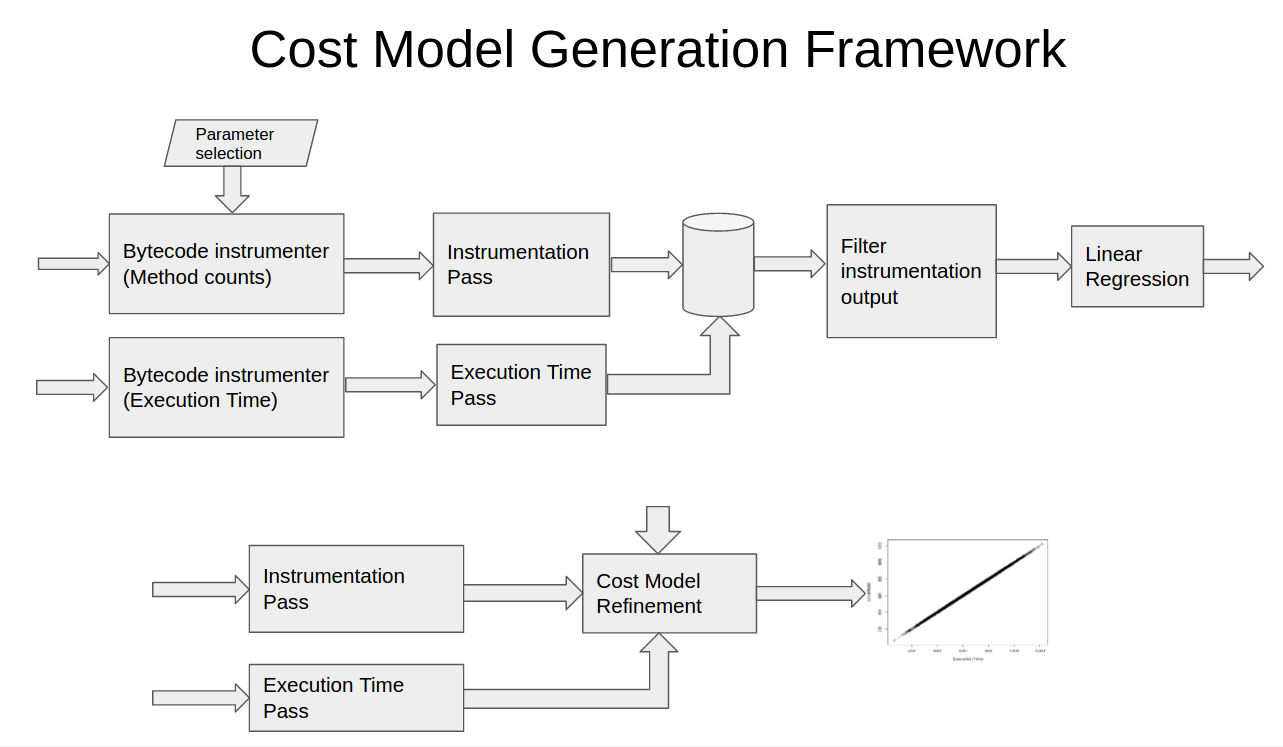
\includegraphics[scale=0.38]{./images/costmodelframework.png}

\subsection{Bytecode Instrumentation}
Bytecode instrumentation is a technique of adding code to compiled classes of a Java application. It is one of the methods to extract profiling information from a Java application. We use it to add code monitoring capabilities to classes without having to modify and recompile source code manually. An instrumenter class injects valid bytecode instructions at specific points of interest within a Java application.\citep{javabytecode}\newline

Java is a dynamically loaded language. Every class is loaded lazily when needed using a component called a class loader. The class loader looks for the class code, reads it, and passes it to the JVM which links it with the rest of the code that is already loaded. This behavior makes Java very flexible – selection of concrete classes is deferred to the last possible moment, and the code itself can be brought from exotic places of all sorts. The basic concept of bytecode instrumentation is to add lines of bytecode before and after specific method calls within a class, and this can be done by intervening with the class loader. 

\subsubsection{Block Instrumenters}

Instrumentation can be performed on the bytecode instruction level, basic block level or the method level.\newline

\textbf{Bytecode instruction level instrumenter}\newline
Instruction level instrumentation is very fine grained and involves inserting bytecode instructions before or after the targeted bytecode instruction. The Shrike utility in WALA and ASM library were the options that were tried to achieve this fine grain instrumentation. Eventually, we settled with using a tool called ByCounter which added a counter for every bytecode instruction present in the source code. This ByCounter needs to be provided with method signatures and canonical class names to perform instrumentation. A driver program was written that would list down all the declared methods within a Java application and its corresponding canonical class name. This was done using WALA core and util packages. \newline

ByCounter application with the driver code is available on GITHUB in the Java-Bytecode-Instrumenter repository. \newline

\textbf{Basic Block level instrumenter}\newline

Basic block instrumenter was written using the Soot framework. It is currently a part of the Exploitr tool on GITHUB. The instrumenter application generates a list of basic blocks which are the ones that are instrumented to get execution counts. Basic blocks are a piece of straight line code sequence with no branches. They have a single entry point and a single exit point.

The list of methods for an application jar is generated using the following command:\newline
\$ java -jar exploitr.jar Test.jar --printMethodCount -d 2

This generates three distinct files consisting of a list of methods, basic blocks and loops respectively. 

\$ java -jar exploitr.jar Test.jar -i blockCodeInstrument -x list\_of\_blocks.txt

This command generates instrumented classes from Test.jar application. These instrumented classes are injected into the application jar.

\textbf{Method level instrumenter}\newline

Method level instrumenter inserts counts within each method that is specified by the list\_of\_methods.txt file. Method level instrumentation is useful in determining which methods of an application are executed for the given set of inputs. The commands used to generated an instrumented set of classes is similar to basic block instrumentation.\\

\$ java -jar exploitr.jar Test.jar --printMethodCount -d 2

This generates three distinct files consisting of a list of methods, basic blocks and loops respectively. 

\$ java -jar exploitr.jar Test.jar -i expFunInstrument -x list\_of\_methods.txt

This command generates instrumented classes from Test.jar application. These instrumented classes are injected into the application jar.

\subsubsection{Execution time Instrumenter}
The execution time instrumenter was written to time the execution of an application for a provided input. System.nanoTime() calls are added to the main method of an application with the help of ASM libraries. The Java application under analysis is given a range of varying inputs and the execution times corresponding to each of these inputs is logged into a csv file. The same inputs are provided to the block instrumenter for generating block invocation counts. \\

\textbf{ASM framework}\newline

ASM uses the visitor pattern. Objects or Acceptors include the ClassReader class and the MethodNode class. Visitor interfaces include ClassVisitor, AnnotationVisitor, FieldVisitor, and MethodVisitor.  ClassReader reads Java Bytecode from a file, and ClassWriter writes Bytecode to a file. ASM is using the Visitor Pattern: ClassWriter implements the of ClassVisitor interface, and the call to cr.accept(cw, 0) causes ClassReader to traverse the Bytecode input, making a series of calls to cw that generate the same Bytecode as output. The ClassWriter.COMPUTE\_FRAMES argument to the ClassWriter constructor is an option flag that indicates we would like the ClassWriter to compute the size of stack frames for us. \newline

In order to modify the classes, we need to insert some code in between ClassReader and ClassWriter. We will do this using the Adapter Pattern. Adapters wrap an object, overriding some of its methods, and delegating to the others. This gives us an easy way to modify the behavior of the wrapped object. We will \@override the behavior of only the ClassWriter.visitMethod method, which is called once for each method declaration in a class. The return value of visitMethod is a a MethodVisitor object, which is used to process the method body. ClassWriter.visitMethod returns a MethodVisitor that produces the Bytecode for a method. We will adapt the MethodVisitor returned by ClassWriter.visitMethod. and insert additional instructions.\\

\textbf{Timing an application}\newline

In the given example code below, the Test class has been instrumented for fetching the execution time of the code using System.nanoTime() methods. These calls are inserted at the start and end of the main method. The MainTransformer class extends GeneratorAdapter and we override two specific methods: visitCode() and visitInsn(). The visitCode() method is visited at the start of the any method. We are aiming for the main method here and hence add a new instance to the MainTransformer only when the MethodVisitor visits the \"main\" method. The visitInsn() method is visited for each bytecode instruction. We specifically look for the \"RETURN\" opcode and add instrumentation just before the return bytecode instruction is executed.\\

We need to add instrumentation using ASM's API. ASM has a package names "ASMifier" which turns Java bytecode instructions to be added into intermediate ASM code that is required for ASM to transform the class. To insert the System.nanoTime() call into the main method we add the following lines to visitCode():

\begin{lstlisting}
super.visitMethodInsn(Opcodes.INVOKESTATIC, "java/lang/System", "nanoTime", 
"()J", false);
super.visitVarInsn(Opcodes.LSTORE, 1);
\end{lstlisting}

Listed below is the complete Instrumenter class which takes a Test class to be transformed as an input argument and instruments the bytecode for measuring total execution time.

\begin{lstlisting}
public class Instrumenter {
    public static void main(final String args[]) throws Exception {
        FileInputStream is = new FileInputStream(args[0]);
        byte[] b;

        ClassReader cr = new ClassReader(is);
        ClassWriter cw = new ClassWriter(ClassWriter.COMPUTE_FRAMES);
        ClassVisitor cv = new ClassAdapter(cw);
        cr.accept(cv, cr.EXPAND_FRAMES);
        b = cw.toByteArray();

        FileOutputStream fos = new FileOutputStream(args[1]);
        fos.write(b);
        fos.close();
    }
}

class ClassAdapter extends ClassVisitor implements Opcodes {

    public ClassAdapter(final ClassVisitor cv) {
        super(ASM5, cv);
    }

    @Override
    public MethodVisitor visitMethod(int access, String name, String desc, 
    String signature, String[] exceptions) {

        MethodVisitor v=super.visitMethod(access, name, desc, signature, 
        exceptions);
        if(name.equals("main") && desc.equals("([Ljava/lang/String;)V"))
        v=new MainTransformer(v, access, name, desc, signature, exceptions);
        return v;
    }
}

class MainTransformer extends GeneratorAdapter
  {
    MainTransformer(MethodVisitor delegate, int access, String name, 
    String desc, String signature, String[] exceptions) {
      super(Opcodes.ASM5, delegate, access, name, desc);
    }

     @Override
     public void visitCode() {

        super.visitMethodInsn(Opcodes.INVOKESTATIC, "java/lang/System", 
        "nanoTime", "()J", false);
        super.visitVarInsn(Opcodes.LSTORE, 1);
        super.visitCode();

     }

    @Override
    public void visitInsn(int opcode) {
      if(opcode==Opcodes.RETURN) {
	super.visitMethodInsn(Opcodes.INVOKESTATIC, "java/lang/System", 
	"nanoTime", "()J", false);
        super.visitVarInsn(Opcodes.LSTORE, 3);
        super.visitVarInsn(Opcodes.LLOAD, 3);
        super.visitVarInsn(Opcodes.LLOAD, 1);
        super.visitInsn(Opcodes.LSUB);
        super.visitVarInsn(Opcodes.LSTORE, 5);
        super.visitVarInsn(Opcodes.LLOAD, 5);
        super.visitInsn(Opcodes.L2D);
        super.visitLdcInsn(new Double("1000000.0"));
        super.visitInsn(Opcodes.DDIV);
        super.visitVarInsn(Opcodes.DSTORE, 7);
        super.visitFieldInsn(Opcodes.GETSTATIC, "java/lang/System", 
        "out","Ljava/io/PrintStream;");
        super.visitTypeInsn(Opcodes.NEW, "java/lang/StringBuilder");
        super.visitInsn(Opcodes.DUP);
        super.visitMethodInsn(Opcodes.INVOKESPECIAL, 
        "java/lang/StringBuilder", "<init>", "()V", false);
        super.visitLdcInsn("\n\rDURATION: ");
        super.visitMethodInsn(Opcodes.INVOKEVIRTUAL, 
        "java/lang/StringBuilder", "append", 	
        "(Ljava/lang/String;)Ljava/lang/StringBuilder;", false);
        super.visitVarInsn(Opcodes.DLOAD, 7);
        super.visitMethodInsn(Opcodes.INVOKEVIRTUAL, 
        "java/lang/StringBuilder", "append", 
        "(D)Ljava/lang/StringBuilder;", false);
        super.visitMethodInsn(Opcodes.INVOKEVIRTUAL,
        "java/lang/StringBuilder", "toString", "()Ljava/lang/String;", false);
        super.visitMethodInsn(Opcodes.INVOKEVIRTUAL, 
        "java/io/PrintStream", "println", "(Ljava/lang/String;)V", false);
      }
      super.visitInsn(opcode);
    }
  }
\end{lstlisting}

The instrumentation used above is better than timing the execution of an application from command line. The command line measurement includes the overhead of JVM startup time. For such measurements, the JIT optimization is turned off and garbage collection is disabled.\\

To instrument the Test class ,run the command given below:

\$ java -cp .:asm-all-5.0.3.jar Instrumenter TestClass.class InstrumentedClass.class

\textbf{Timing Basic Blocks}\newline

This approach is contrary to the one where we would instrument an application for basic block counts and classify these based on the total execution time. Here, we are following a fine grain approach where we are going to time each basic block within an application. A list of basic blocks to be timed is obtained from the exploitr tool. ASM is used to add instrumentation at the head and tail of each basic block in the list where a head represents the starting bytecode index of the basic block and tail represents the ending bytecode index. The MainTransformer class for this experiment is presented below:

\begin{lstlisting}
class MainTransformer extends GeneratorAdapter
  {
    MainTransformer(MethodVisitor delegate, int access, String name, 
     String desc, String signature, String[] exceptions) {
      super(Opcodes.ASM5, delegate, access, name, desc);
    }


    @Override
    public void visitLineNumber(int line, Label start) {

        HashMap<Integer, String> blockMap = new HashMap<Integer, String>();
        System.out.println(line);
        if(blockMap.get(line) != null){
           if(blockMap.get(line) == "head"){
               super.visitFieldInsn(Opcodes.GETSTATIC, 
               "java/lang/System", "out", "Ljava/io/PrintStream;");
               super.visitVarInsn(Opcodes.ILOAD, 1);
               super.visitMethodInsn(Opcodes.INVOKEVIRTUAL, 
               "java/io/PrintStream", "println", "(I)V", false);
               super.visitMethodInsn(Opcodes.INVOKESTATIC, 
               "java/lang/System", "nanoTime", "()J", false);
               super.visitVarInsn(Opcodes.LSTORE, 1);
           }
           else if(blockMap.get(line) == "tail"){
                super.visitFieldInsn(Opcodes.GETSTATIC, 
                "java/lang/System", "out", "Ljava/io/PrintStream;");
                super.visitVarInsn(Opcodes.ILOAD, 1);
                super.visitMethodInsn(Opcodes.INVOKEVIRTUAL, 
                "java/io/PrintStream", "println", "(I)V", false);
                super.visitMethodInsn(Opcodes.INVOKESTATIC, 
                "java/lang/System", "nanoTime", "()J", false);
                super.visitVarInsn(Opcodes.LSTORE, 3);
                super.visitVarInsn(Opcodes.LLOAD, 3);
                super.visitVarInsn(Opcodes.LLOAD, 1);
                super.visitInsn(Opcodes.LSUB);
                super.visitVarInsn(Opcodes.LSTORE, 5);
                super.visitVarInsn(Opcodes.LLOAD, 5);
                super.visitInsn(Opcodes.L2D);
                super.visitLdcInsn(new Double("1000000.0"));
                super.visitInsn(Opcodes.DDIV);
                super.visitVarInsn(Opcodes.DSTORE, 7);
                super.visitFieldInsn(Opcodes.GETSTATIC, 
                "java/lang/System", "out", "Ljava/io/PrintStream;");
                super.visitTypeInsn(Opcodes.NEW, 
                "java/lang/StringBuilder");
                super.visitInsn(Opcodes.DUP);
                super.visitMethodInsn(Opcodes.INVOKESPECIAL, 
                "java/lang/StringBuilder", "<init>", "()V", false);
                super.visitLdcInsn("\n\rDURATION: ");
                super.visitMethodInsn(Opcodes.INVOKEVIRTUAL, 
                "java/lang/StringBuilder", "append", 
                "(Ljava/lang/String;)Ljava/lang/StringBuilder;", false);
                super.visitVarInsn(Opcodes.DLOAD, 7);
                super.visitMethodInsn(Opcodes.INVOKEVIRTUAL, 
                "java/lang/StringBuilder", "append", 	
                "(D)Ljava/lang/StringBuilder;", false);
                super.visitMethodInsn(Opcodes.INVOKEVIRTUAL, 
                "java/lang/StringBuilder", "toString", 
                "()Ljava/lang/String;", false);
                super.visitMethodInsn(Opcodes.INVOKEVIRTUAL, 
                "java/io/PrintStream", "println", 
                "(Ljava/lang/String;)V", false);
            }
        }
        super.visitLineNumber(line, start);
    }

  }
\end{lstlisting}

To instrument the Test class ,run the command given below:

\$ java -cp .:asm-all-5.0.3.jar BasicBlockInstrumenter TestClass.class InstrumentedClass.class

The instrumented class will output the basic block identifier with the end index as the key and the timing value. This timing functionality was used to test if we could time basic blocks in this manner and get accurate results as compared to the Cost Model approach.

\subsubsection{Memory Usage Instrumenter}
The memory usage instrumenter profiles Java bytecode to get the total memory usage of an application. Memory usage of a Java program, at the very basic level, can be obtained with the following code:
\begin{lstlisting}
Runtime runtime = Runtime.getRuntime();
long memoryBefore = runtime.totalMemory() - runtime.freeMemory();

..... code here .....

long memoryAfter = runtime.totalMemory() - runtime.freeMemory();
System.out.print("MEMORY:");
System.out.println((memoryAfter - memoryBefore)/(1024L));
\end{lstlisting}

The class transformer shown below presents this source in ASM format:

\begin{lstlisting}
class MainTransformer extends GeneratorAdapter
  {
    MainTransformer(MethodVisitor delegate, int access, String name,
     String desc, String signature, String[] exceptions) {
      super(Opcodes.ASM5, delegate, access, name, desc);
    }


    @Override
    public void visitInsn(int opcode) {
      if(opcode==Opcodes.RETURN) {
        super.visitMethodInsn(Opcodes.INVOKESTATIC, "java/lang/Runtime", 	
        "getRuntime", "()Ljava/lang/Runtime;", false);
        super.visitVarInsn(Opcodes.ASTORE, 1);
        super.visitVarInsn(Opcodes.ALOAD, 1);
        super.visitMethodInsn(Opcodes.INVOKEVIRTUAL, "java/lang/Runtime", 
        "totalMemory", "()J", false);
        super.visitVarInsn(Opcodes.ALOAD, 1);
        super.visitMethodInsn(Opcodes.INVOKEVIRTUAL, "java/lang/Runtime", 
        "freeMemory", "()J", false);
        super.visitInsn(Opcodes.LSUB);
        super.visitVarInsn(Opcodes.LSTORE, 2);
        super.visitFieldInsn(Opcodes.GETSTATIC, "java/lang/System", "out", 
        "Ljava/io/PrintStream;");
        super.visitVarInsn(Opcodes.LLOAD, 2);
        super.visitLdcInsn(new Long(1024L));
        super.visitInsn(Opcodes.LDIV);
        super.visitMethodInsn(Opcodes.INVOKEVIRTUAL, "java/io/PrintStream", 
        "println", "(J)V", false);
      }
      super.visitInsn(opcode);
    }
  }
\end{lstlisting}

Memory Instrumenter is subject to errors due to garbage collection in Java and would not always be accurate. The heap size and stack size could be made large enough to delay the garbage collection until these memory regions are fully occupied. 

\subsection{Estimation using Multiple Linear Regression}
We need to estimate the time per block for a given Java application. The Multiple Linear regression takes \textbf{time} as the dependent variable and \textbf{blocks} as independent variables. The estimates can be applied to predict execution time of applications that make use of these methods.\newline 

\textbf{Multiple Linear Regression}\\

Multiple linear regression attempts to model the relationship between two or more explanatory variables and a response variable by fitting a linear equation to observed data.\citep{linearreg} Every value of the independent variable x is associated with a value of the dependent variable y. It is applicable to numerous data mining situations. Examples are: predicting customer activity on credit cards from demographics and historical activity patterns, predicting the time to failure of equipment based on utilization and environment conditions.The values of the independent variables(also referred to as predictor variables, regressors or covariates) are known quantities for purposes of prediction, the model is:

\begin{equation}
Y = \beta_{0} + \beta_{1}X_{1}+ \beta_{2}X_{2} + \dotsb+ \beta_{n}X_{n} + \epsilon
\end{equation}

where $\beta_{n}$ are the regression coefficients or estimates\\
$X_{n}$ are the block invocation counts\\
$\epsilon$ is the normally distributed "noise" random variable

The data consist of n rows of observations also called cases, which give us values $y_{i},x_{i1},x_{i2},x_{ip}$; i = 1,2,..n.  The estimates for the $\beta$ coefficients are computed so as to minimize the sum of squares of differences between the fitted (predicted) values at the observed values in the data.\\

The estimates obtained from regression analysis can be used to predict total execution time of test applications which use these blocks/methods. 

\textbf{Script for linear regression}:
\begin{lstlisting}
args <- commandArgs(TRUE)
x = read.csv(args[1], header=TRUE)
full = lm(ExecTime ~ . - 1, data = x)
stepResults = step(full, data=x, direction="backward")
coefficients(stepResults)
summary(full)
m = as.matrix(coefficients(full))
m[is.na(m)] <- 0
y = read.csv(args[2], header = TRUE)
a = as.matrix(within(y, rm('ExecTime')))
LinearModel = as.matrix(a %*% m)
ExecutionTime = as.matrix(y['ExecTime'])
plot(ExecutionTime, LinearModel)
\end{lstlisting}

The command to run Linear Regression over the application data consisting of block invocation counts is given below:

\$ ./LinearRegression.R blockTrainingData.csv blockTestData.csv

where blockTrainingData.csv is the training data set
	  blockTestData.csv is the test data set
	  
The "lm" function takes in a dependent variable and a set of independent variables. The dependent variable here is ExecTime and the independent variables are all the blocks/methods within the data file. The linear regression output of lm lists down the coefficients for each block. These coefficients provide an estimate of time per block. Standard error, residuals and the R-squared value are some other parameters than provide the goodness of a fit using regression. The "step" function is used as a mechanism for subset selection out of the available blocks as independent variables.
Once the estimates are calculated from the training data set, these can be applied to the test data set and we can check how well the model fits the test set. The test data consists of block invocation counts. The corresponding execution time can also be measured in order to check if the training set works well. On plotting the predicted time and the actual execution time, the resulting plot should be linear for the model to be a good fit.
\newpage

\textbf{Non negative least squares}\\

The regression coefficients from lm function can be negative. The regression algorithm decides the best fit possible and the coefficients for some independent variables could turn out negative.\citep{nnls} Time as a physical quantity cannot be negative and hence we want to force the coefficients to be positive. In doing this, we may make some of the coefficients to be zero.

\textbf{Script for NNLS regression}

\begin{lstlisting}
args <- commandArgs(TRUE)
x = read.csv(args[1], header=TRUE)
a = as.matrix(within(x, rm('ExecTime')))
a[is.na(a)] <- 0
b = as.matrix(x['ExecTime'])
b[is.na(b)] <- 0
library(nnls)
y = nnls(a, b)
coefficients(y)
m = as.matrix(coefficients(y))
m[is.na(m)] <- 0
z = read.csv(args[2], header = TRUE)
a1 = as.matrix(within(z, rm('ExecTime')))
PredictedTime = as.matrix(a1 %*% m)
ExecTime = as.matrix(z['ExecTime'])
plot(ExecTime, PredictedTime)
\end{lstlisting}

This script works in a similar manner as the linear regression script. Here, instead of "lm" we use "nnls" function to calculate regression coefficients.

For our final tool, we have been using linear regression script as the NNLS method forces quite a few useful coefficients to be zero. The estimation information extracted out of the NNLS method is lesser. There is no control over which coefficients are forced to be zero by the algorithm. Instead, we have worked on refinement of the linear regression method to have the perfect fit such that it does not produce negative coefficients.
\newpage

\section{Results}
Cost Model Tool can provide information about estimation coefficients of methods/basic blocks used in Java applications. It can also be used with the training and testing approach where we try to check if a training set of applications fits an application under test. Since we have tried our model at various levels of an application, we will be discussing results separately for instruction level disambiguation, method level disambiguation and block level disambiguation.

\subsection{Bytecode Instruction disambiguation}
The bytecode instruction disambiguation results for Arithmetic applications having operations add, subtract, multiply, divide are discussed in this report.

Bytecodes are a huge set of instructions. They have high correlation between them. Using our bytecode instrumenter, we were able to capture the executed bytecode instructions for a given input. Arithmetic applications gave us a target set of bytecodes which could be considered as buckets for regression analysis.\citep{bytecodetiming}

\textbf{Linear regression}

Call:\\
lm(formula = Time ~ . - 1, data = x)

Residuals:\\
Min\hspace{4em}1Q\hspace{4em}Median\hspace{3em}3Q\hspace{4em}Max \\
-0.03187\hspace{2em}-0.01919\hspace{2em}-0.00678\hspace{2em}0.00800\hspace{2em}0.33727 

Coefficients: (2 not defined because of singularities)\\

\begin{table}[h!]
\begin{center}
 \begin{tabular}{ |c|c|c|c|c| }
 \hline
 Opcodes&Estimate&Std. Error&t value&Pr()    \\
 \hline
 SUB&-1.759e-06&3.553e-07&-4.952&7.97e-07 ***\\
 CALLS&6.401e-03&1.280e-03&5.0030&6.15e-07 ***\\
 LDST&1.319e-06&3.585e-08&36.804&2e-16 ***\\
 ADD&-2.097e-06&3.536e-07&-5.930&3.56e-09 ***\\
 OTHERS&NA&NA&NA&NA\\
 MUL&-2.339e-06&3.513e-07&-6.659&3.55e-11 ***\\
 DIV&NA&NA&NA&NA\\ 
 \hline
 \end{tabular}
\end{center}
\caption{Estimates for opcodes executed in Java application}
\label{Linear Regression results:1}
\end{table}

Signif. codes:  0 ‘***’ 0.001 ‘**’ 0.01 ‘*’ 0.05 ‘.’ 0.1 ‘ ’ 1

Residual standard error: 0.03236 on 1994 degrees of freedom\\
Multiple R-squared:  0.9959 \hspace{2em} Adjusted R-squared:  0.9959 \\
F-statistic: 9.632e+04 on 5 and 1994 DF,  p-value: 2.2e-16\\

Applying linear regression to the data generated from arithmetic bytecode instructions results in negative coefficients for certain bytecodes like SUB, ADD and MUL. The bucketing of bytecode counts has been performed as per the following categorization:\\
\begin{lstlisting}
ADD           - ADD
SUBTRACT      - SUB
MULTIPLY      - MUL
DIVIDE        - DIV
CALLS         - Method Calls
LDSTCOND      - LOAD,STORE,PUSH,POP,GETSTATIC,CONST,IFEQ,GOTO,ICMP,INC,I2D
\end{lstlisting}

The negative coefficients are a result of the existence of high correlation among the various bytecode opcodes. Subset selection of opcode buckets has been used in the Linear regression script to get the perfect fitting for a given set of buckets. However, the negative coefficients still remain. We have not been able to completely eliminate the negative coefficients as the bytecodes have a strong correlation however, we cannot directly remove certain buckets as these appear individually as well. For example, LOADs and STOREs accompany the arithmetic instructions. However, these can appear independently as well and hence completely eliminating them can introduce an error in the final estimation. The time taken by these bytecodes will go into some other bucket. This can cause the linear fitting algorithm to make certain buckets very strong and have a positive coefficient for these while make certain buckets weaker and subsume the fitting error out of these. Hence, we were not able to disambiguate bytecode instructions entirely. 

We have used a new approach which applies non negative least squares algorithm to the data. The results from this algorithm have been presented below.

\textbf{NNLS} \newline
\begin{table}[h!]
\begin{center}
\begin{tabular}{|c|c|c|c|c|}
\hline
SUB&CALLS&ADD&MUL&DIV\\
\hline
7.4768e-06&0.006411&7.1393e-06&6.8969e-06&9.2361e-06 \\
\hline
\end{tabular}
\end{center}
\caption{Non negative least squares model}
\label{NNLS  results:2}
\end{table}

residual sum-of-squares: 2.088

As it can be observed from the results, this algorithm does provide positive coefficients for the results. The mean squared error seen from the residual sum of squares is quite less and we can consider this disambiguation as a good estimation of the arithmetic bytecode instructions. 

We were able to achieve this by removing all other type of instructions and method calls from the training program. However, this algorithm NNLS has a tendency to force certain buckets to zero. This may lead to loss of information on our part. For this particular bytecode disambiguation program, NNLS has worked well. However, for regression analysis in later section, we will be switching back to the linear regression algorithm as it seems to be more reliable.

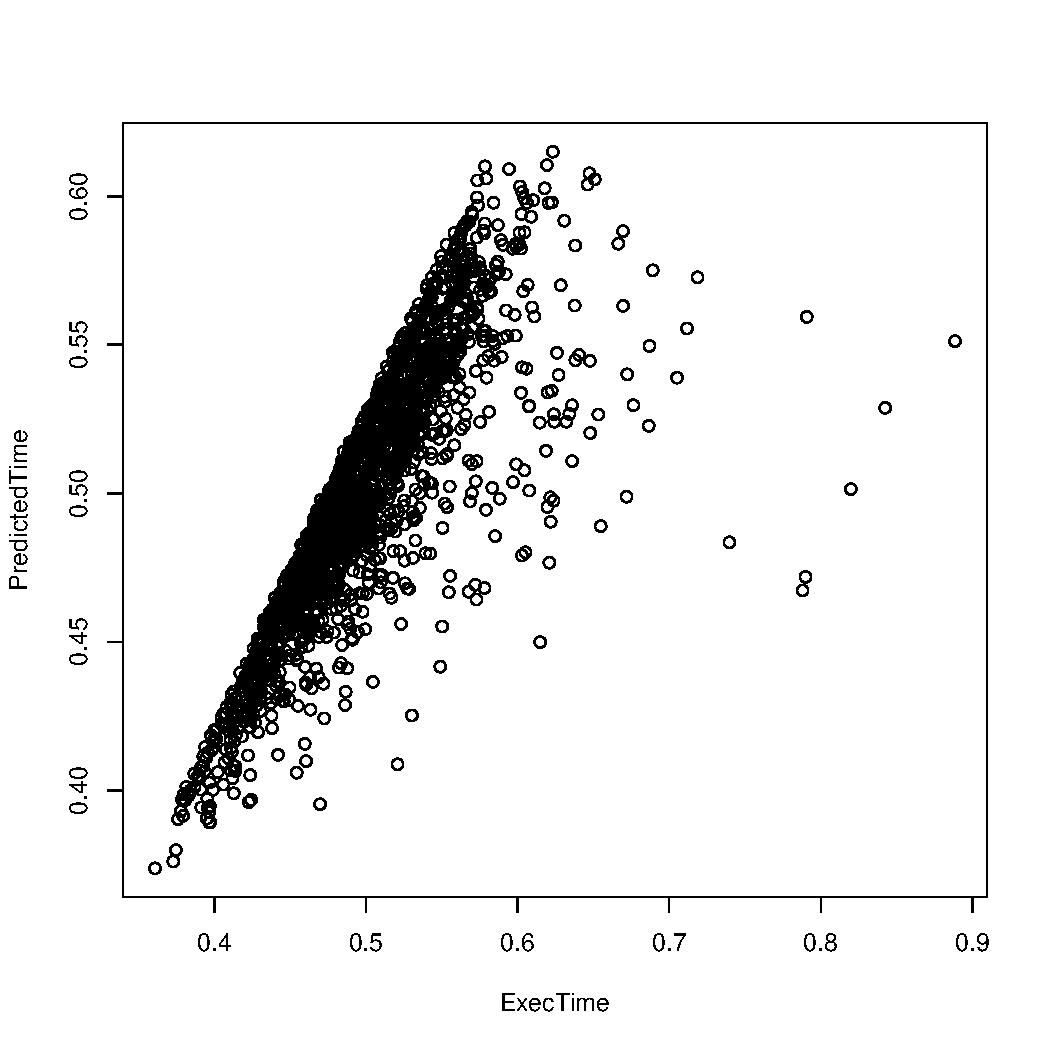
\includegraphics[scale=0.7]{Rplots.pdf}

In the above plot, time predicted using a training model for an application has been plotted against the actual measured execution time for the same application. As it can be seen, the plot is linear with the scales matching. This is a good indicator that the predicted time is accurate. Prediction using this cost model have been successful only on arithmetic rich applications. For other applications, this model does not produce a linear plot.
\newpage

\subsection{Method disambiguation}
This section includes the results of method level disambiguation on Java applications. 

\textbf{Result 1}

This set of results relates to a Java application having methods with no branches and mere sleep calls within the source code. The code can be checked within the Method disambiguation section of chapter Motivating Examples. 

lm(formula = Time ~ . - 1, data = x)

Residuals:\\
Min\hspace{4em}1Q\hspace{4em}Median\hspace{3em}3Q\hspace{4em}Max \\
-0.24089\hspace{2em}-0.05356\hspace{2em}-0.00746\hspace{2em}0.03857\hspace{2em}1.23960 

Coefficients:\\
\begin{table}[h!]
\begin{center}
 \begin{tabular}{ |c|c|c|c|c| }
 \hline
 Opcodes&Estimate&Std. Error&t value&Pr()    \\
 \hline
Function1&1.131e+00&1.572e-03&719.77&2e-16 ***\\
Function2&1.014e+01&2.511e-03&4036.13&2e-16 ***\\
Function3&5.002e+02&1.588e-03&315008.55&2e-16 ***\\
Function4&1.002e+02&2.172e-03&46108.56&2e-16 ***\\
Function5&2.807e-02&1.948e-03&14.41&2e-16 ***\\
 \hline
 \end{tabular}
\end{center}
\caption{Estimates for opcodes executed in Java application}
\label{Linear Regression results:3}
\end{table}

Signif. codes:  0 ‘***’ 0.001 ‘**’ 0.01 ‘*’ 0.05 ‘.’ 0.1 ‘ ’ 1

Residual standard error: 0.08715 on 1993 degrees of freedom\\
Multiple R-squared:      1\hspace{2em}Adjusted R-squared:      1\\ 
F-statistic: 2.925e+10 on 5 and 1993 DF,  p-value: 2.2e-16

We can clearly see here that the estimation coefficients make perfect sense. The delays introduced in each of these functions have been predicted accurately by the linear regression algorithm. 

\textbf{Result 2}

The application under test in result 1 did not have any branches within the methods. The result being presented here belongs to the example application 3.3.1 that has been discussed in the cost estimation chapter. 

\textbf{Linear Regression}

lm(formula = ExecTime ~ . - 1, data = x)\\

Residuals:\\
Min\hspace{4em}1Q\hspace{4em}Median\hspace{3em}3Q\hspace{4em}Max \\
-0.25052\hspace{2em}-0.07541\hspace{2em}-0.04494\hspace{2em}0.04426\hspace{2em}0.71142 

Coefficients: (1 not defined because of singularities)\\
\begin{table}[h!]
\begin{center}
 \begin{tabular}{ |c|c|c|c|c| }
 \hline
 Opcodes&Estimate&Std. Error&t value&Pr()    \\
 \hline
X.MainClass..void.func4...&100.16798&0.02224&4504.892&2e-16 ***\\
X.MainClass..int.bubbleSort.int..&0.29618&0.03839&7.715&6.32e-13 ***\\
X.MainClass..void.QuickSort.int..&-0.03262&0.01723&-1.893&0.0598\\
X.MainClass..void.func7...&20.48876&0.04669&438.828&2e-16 ***\\
X.MainClass..void.func3.int..&0.92409&0.01966&47.006&2e-16 ***\\
X.MainClass..void.func6...&20.25167&0.01777&1139.750&2e-16 ***\\
X.MainClass..void.func5...&NA&NA&NA&2e-16 ***\\
\hline
\end{tabular}
\end{center}
\caption{Estimates for opcodes executed in Java application}
\label{Linear Regression results:4}
\end{table}

Signif. codes:  0 ‘***’ 0.001 ‘**’ 0.01 ‘*’ 0.05 ‘.’ 0.1 ‘ ’ 1

Residual standard error: 0.1274 on 193 degrees of freedom\\
Multiple R-squared:      1\hspace{2em}Adjusted R-squared:      1 \\
F-statistic: 8.411e+06 on 6 and 193 DF,  p-value: 2.2e-16

From the results, we can see that linear regression does not apply well to methods that have branches inside and are more complicated in terms of one method calling another. Some of these methods take constant time while for some others the amount of execution time is dependent on branches. 

I have tried an approach where only the list of methods whose execution time is required, are given to the instrumenter. This deletion of irrelevant methods will vary from application to application and cannot be automated. However, even after removing irrelevant methods, there are some coefficients that appear negative. Due to this, we explored another approach where we can present the dependent and independent variables in the form of a matrix as equations. The idea is to find a unique solution for a certain set of equations from the data file. Given below is the script used to get unique solutions for independent linear equations.
\newpage

\begin{lstlisting}
> x=read.csv(args[1],header=TRUE)
> a = as.matrix(within(x, rm('ExecTime')))
> a[is.na(a)] <- 0
> b = as.matrix(x['ExecTime'])
> b[is.na(b)] <- 0
> solve(a,b)
\end{lstlisting}

\begin{table}
\begin{center}
\begin{tabular}{|c|c|}
\hline         
Functions&Execution Time\\ 
\hline
X.MainClass..void.func4&100.097646\\
X.MainClass..int.bubbleSort.int...int.int&0.510821\\
X.MainClass..void.QuickSort.int...int.int&0.075028\\
X.MainClass..void.func7&20.100512\\
X.MainClass..void.func3.int&1.119532\\
X.MainClass..void.func6&20.099019\\
\hline
\end{tabular}
\caption{Linear Equation Solving results}
\end{center}
\end{table}

As we can see from the results, the estimates are non negative. They match with the complexity of code within each method. This approach provides a good disambiguation on the method level. The Equation solving construct identifies inputs that are independent of one another. This produces a unique solution for that set of equations.

On testing further, it can be said that this approach of solving linear system of equations works well with smaller applications i.e. applications having a small set of methods. When there is a large set of methods, it is required to produce independent inputs equal to the number of methods under analysis. Only then can the linear system of equations identify the inputs and use its data to get unique estimates.
\newpage

\subsection{Basic block disambiguation}
Basic blocks are most fundamental units of code. They represent straight line code without any jumps. We mentioned a problem with methods that the execution time for each method cannot be constant. This is because a branch within a method may take more time to execute than another branch. There is a need to disambiguate the imbalance due to these paths. This is where basic blocks are useful. Like methods, one can identify all basic blocks within an application and instrument the code to add a counter for each basic block. Basic blocks will take constant time to execute. Hence, the idea of having a cost model for basic blocks sounds right.

In this section, I will be presenting results for basic block disambiguation using two approaches: fine grain timing and cost model

\textbf{Result 1: Fine grain timing}

Fine grain timing involves inserting timing calls at the start and end of each basic block. Please refer to section 2.1.1 for source code. The results obtained from this experiment are as below:

\textbf{Run 1:}

Execution time measurements in milliseconds(ms):\\
\\Basic block 1: 0.440963 \\
\\Basic block 2:\\
\hspace{2em} Iteration 1: 0.332355\\
\hspace{2em} Iteration 2: 0.0012\\
\hspace{2em} Iteration 3: 0.001012\\
\hspace{2em} Iteration 4: 0.000965\\
\hspace{2em} Iteration 5: 0.000966\\
\hspace{2em} Iteration 6: 0.000887\\
\hspace{2em} Iteration 7: 0.000926\\
\hspace{2em} Iteration 8: 0.000914\\
\\Basic block 3: 1.11022\\

\textbf{Run 2:}

Execution time measurements in milliseconds(ms):\\
\\Basic block 1: 0.318824\\
\\Basic block 2:\\
\hspace{2em} Iteration 1: 0.310898\\
\hspace{2em} Iteration 2: 0.001169\\
\hspace{2em} Iteration 3: 0.001046\\
\hspace{2em} Iteration 4: 0.000961\\
\hspace{2em} Iteration 5: 0.000945\\
\hspace{2em} Iteration 6: 0.000895\\
\hspace{2em} Iteration 7: 0.000904\\
\hspace{2em} Iteration 8: 0.000867\\
\\Basic block 3: 1.086663

\textbf{Statistics}\\

\begin{center}
\begin{tabular}{|c|c|c|c|}
\hline
Blocks&Mean&Standard Deviation&Variance\\
\hline
Basic block 1&0.34247&0.06613&0.00437\\
Basic block 2&0.34247&0.06613&0.00437\\
Basic block 3&1.09533&0.01053&0.00011\\
\hline
\end{tabular}
\end{center}

\textbf{Comments}

From the basic block timing results we see that there is some variance in the measurements of basic block 2. The goal of this experiment was to check if we can time basic blocks accurately. If the timing of basic blocks works accurately, we don't need the cost model approach. Here, we see that there is some variance in the timing a major part of which is due to the first iteration over the basic block. If we neglect the first iteration, the variance is very low. However, we cannot conclude that the basic block timing will work for all applications. It would have some non deterministic elements like the role of JVM, platform on which the experiments are run and so on. Hence, we would like to now check the results using the cost model approach.

\textbf{Result 2: Cost Model estimation}

The cost model approach consists of two passes as we know. The first pass is to get the total execution time for a certain input and the second pass is to get the basic block invocation counts. Over the data generated for a huge set of inputs, we run linear regression and get the results presented below. For source code, please refer to section 2.1.2.

lm(formula = ExecTime ~ . - 1, data = x)

Residuals:\\
Min\hspace{4em}1Q\hspace{3em}Median\hspace{3em}3Q\hspace{3em}Max \\
-0.2459\hspace{2em}-0.0366\hspace{2em}-0.0123\hspace{2em}0.0942\hspace{2em}3.2615\\ 
Coefficients:\\
\begin{table}[h!]
\begin{center}
 \begin{tabular}{ |c|c|c|c|c| }
 \hline
 Opcodes&Estimate&Std. Error&t value&Pr()    \\
 \hline
 X.Test3..void.main.java.lang.String...25&0.0096788&0.0002356&41.08&2e-16 ***\\
 X.Test3..void.main.java.lang.String...15&0.2438942&0.0115409&21.13&2e-16 ***\\
 X.Test3..void.main.java.lang.String...32&1.2122846&0.0101405&119.55&2e-16 ***\\
 \hline
 \end{tabular}
 \end{center}
 \caption{Estimates for basic blocks}
 \label{Linear Regression results:5}
 \end{table}
 
 Signif. codes:  0 ‘***’ 0.001 ‘**’ 0.01 ‘*’ 0.05 ‘.’ 0.1 ‘ ’ 1

Residual standard error: 0.1556 on 1596 degrees of freedom\\
Multiple R-squared:  0.9851\hspace{2em}Adjusted R-squared:  0.9851 \\
F-statistic: 3.522e+04 on 3 and 1596 DF,  p-value:  2.2e-16\\

\textbf{Comments}

Basic block timings estimated using the cost model and linear regression approach have been shown in the results. The estimates are non negative and have a low standard error. The R-squared value is also quite high which denotes this is a good fit and hence it would be fine to disambiguate the three basic blocks using coefficients generated as time per block. This was a small program which worked like a proof of concept. The next result consists of a larger application with multiple method invocations and increased complexity.\\

\textbf{Result 3: Complex application with method invocations}

Here, I am discussing the results of the application listed in section 3.3.1. This application consists of nested function calls, sort implementations of differing complexity. Below are the results that were obtained by running the basic block level cost model on the application:

lm(formula = ExecTime ~ . - 1, data = x)

Residuals:\\
Min\hspace{3.5em}1Q\hspace{3em}Median\hspace{3em}3Q\hspace{3em}Max \\
-43.239\hspace{2em}-1.424\hspace{2em}-0.182\hspace{2em}22.229\hspace{2em}25.177\\
Coefficients:
\begin{table}[h!]
\begin{center}
 \begin{tabular}{ |c|c|c|c|c| }
 \hline
 Opcodes&Estimate&Std. Error&t value&Pr()    \\
 \hline
X.MainClass..int.function2.int....139&48.0102&1.6867&28.464&2e-16 ***\\
X.MainClass..int.function5.....37&0.3529&0.7988&0.442&0.659\\    
X.MainClass..int.function2.int....147&47.8957&1.9894&24.076&2e-16 ***\\
X.MainClass..void.function3.....25&499.7834&1.1207&445.949&2e-16 ***\\
X.MainClass..void.function1.....19&0.5975&0.8676&0.689&0.491\\    
X.MainClass..void.function4.....31&101.2597&1.5948&63.494&2e-16 ***\\
\hline
 \end{tabular}
 \end{center}
 \caption{Estimates for basic blocks within functions}
 \label{Linear Regression results:6}
 \end{table}
 
Signif. codes:  0 ‘***’ 0.001 ‘**’ 0.01 ‘*’ 0.05 ‘.’ 0.1 ‘ ’ 1

Residual standard error: 24.08 on 993 degrees of freedom\\
Multiple R-squared:  0.9988\hspace{2em}Adjusted R-squared:  0.9988\\ 
F-statistic: 1.359e+05 on 6 and 993 DF,  p-value: $<$ 2.2e-16\\

\textbf{Comments}

For this example, we have not instrumented all the basic blocks in the application but a few interesting ones. The estimates calculated for block at line 25, line 31, line 19 and line 37 look accurate. The basic blocks at line 139 and 147 are the ones that need to be analysed. BB at line 139 calls a bubbleSort sorter to sort an array of upto 200 numbers and BB at line 147 calls a quickSort sorter to sort the same array of 200 numbers. As it can be seen, quickSort takes a little lesser time than bubbleSort. This difference would have been more prevalent if the size of the input array was large. Hence, we can conclude that the basic block approach does remove the problem with branching in methods. However, the problem of correlation between blocks or methods still remains. This can be eliminated by manually selected the relevant and uncorrelated buckets or by using some algorithm which filters the list of methods or basic blocks. \\

\textbf{Note: }Although this algorithm works well on small numbers of methods/basic blocks, removing correlated buckets from large applications is still an open problem which leads to negative estimates/coefficients for the buckets.
\newpage

\section{Future steps}
This report lists quite a few problems with the cost model tool due to which the prediction or estimation is not always accurate. Here, I have identified two specific areas which can significantly improve the strike rate of our cost model: test input generation and non linear regression. The next extension would be to have a cost model for space. Once the estimation techniques have been fixed for a timing cost model, it would be much easier to apply these in the spatial domain and get estimates with respect to memory usage.

\subsection{Test input generation}
Automatic test input generation having a high coverage over all paths within an application is an open research area. Having a tool which generates an input for any given program is one possibility that could solve many problems not only in the cost model approach but also in dynamic analysis of applications and areas like finding security bugs within an application. Finding a bad input out of the many valid inputs is a trivial problem for security applications. Inputs covering a large portion of control flow paths within the application are required to have as many independent executions as we can for the linear regression to work well.

Automatic input generation tools exist, however these do not work well for every type of input. I have noticed that most input generation tools work well with integer or float types. Also, they generate inputs not for an application but for a specific method within the application. A user needs to provide a seed input which is used by the tool to execute different symbolic paths. 

Java PathFinder (JPF) and jCUTE are some of the existing symbolic execution tools. JPF has a symbolic execution extension which helps generate constraints and test inputs for a method within an application.\citep{jpftut}

\subsection{Non linear regression}
Until now, we have tried linear regression to estimate the coefficients (time) of independent variables i.e. blocks or methods within an application. Linear regression looks for a linear relationship between the independent variables and the dependent variable. However, it is quite possible that bytecode executions of Java applications have a nonlinear relationship with time or a relation having both linear and nonlinear components. Since we cannot ignore the nonlinear components, we should try to find which model fits best to an application and extract coefficients for both linear and nonlinear components.

Nonlinear regression is a form of regression analysis in which observational data are modeled by a function which is a nonlinear combination of the model parameters and depends on one or more independent variables. The data are fitted by a method of successive approximations. In non-linear regression the analyst specify a function with a set of parameters to fit to the data. The most basic way to estimate such parameters is to use a non-linear least squares approach which basically approximate the non-linear function using a linear one and iteratively try to find the best parameter values. \citep{nonlinearreg}

Finding good starting values is very important in non-linear regression to allow the model algorithm to converge. If you set starting parameters values completely outside of the range of potential parameter values the algorithm will either fail or it will return non-sensical parameter like for example returning a growth rate of 1000 when the actual value is 1.04. The best way to find correct starting value is to “eyeball” the data, plotting them and based on the understanding that you have from the equation find approximate starting values for the parameters. 

The NLS function in R can be used to perform nonlinear regression. It is necessary to provide a model to the nls function i.e. an equation and a start value for the coefficients. Given below is an example code for nonlinear regression analysis.

\begin{lstlisting}
args <- commandArgs(TRUE)
x=read.csv(args[1],header=TRUE)
m<-nls(time ~ k1*(a * log(a))+k2 , data = x, start=list(k1=10,k2=8))
summary(m)
mean(residuals(m)^2)
\end{lstlisting}

In the above example code, we are reading the data from a file passed as an argument. It has two parameters: a dependent variable "time" and an independent variable "a". In this example, we are trying to model time using an expression consisting of "a". The summary prints the resulting coefficient k1 and k2 and the residuals from the model. 

\subsection{Cost model for memory}
The cost model for memory is an extension of the time based cost model. An application can be instrumented for memory usage (heap usage) by the instrumenter. We need to turn off garbage collection and use the System.runtime() calls to get the memory usage at runtime. Section 4.1.3 talks about a memory instrumenter for Java programs and presents some example code.

With this tool, I haven't tried any experiments with the memory cost model. However, this seems the next logical step to take in resource usage disambiguation for Java programs.

\newpage

\section{Conclusion}
With cost model mining, a number of approaches for bytecode disambiguation namely instruction level, method level and basic block level, have been explored. For calculating estimates multiple linear regression and linear equation solvers have been used. It can be said that each of the disambiguation approaches have a set of target applications on which they work fine. We have been successful in developing a cost model for Java applications with certain limitations.

Bytecode disambiguation is easier if we are working with a class of applications which are using the same kind of bytecodes over and over again. Arithmetic applications have been explored in my study. However, the same could be true for memory accesses, network I/O and so on. Method disambiguation works great if we have straight line code within the application or constant time methods. Basic block disambiguation ideally should work on any applications. It has been shown in the results that it works well with small applications. However, with larger applications the estimates are not totally reliable.

Linear Regression is a fine approach for estimation of execution time for bytecode. It is required that that data fed to a linear regression engine should be such that  buckets are uncorrelated, should not have irrelevant buckets and should have significant amount of code coverage which would guarantee existence of independent inputs. Input generation still remains a grey area and this needs to be explored to achieve complete success in cost model mining.

Prediction of time or space channels for Java bytecode is difficult due to non determinism introduced by the JVM. Cost model mining provides a good mechanism to solve this mystery and disambiguate bytecode on various levels.

\newpage

\begin{thebibliography}{9}
\bibitem{energydisag} 
J. Zico Kolter, Siddarth Batra, Andrew Y. Ng. 
\textit{Energy Disaggregation via Discriminative Sparse Coding}.
 
\bibitem{jvm} 
JVM Internals, blog. \\
\texttt{http://blog.jamesdbloom.com/JVMInternals.html}.

\bibitem{javabytecode} 
Instrumenting Java Bytecode with ASM. \\ 
\texttt{http://web.cs.ucla.edu/~msb/cs239-tutorial/}.

\bibitem{linearreg}
MIT OpenCourseWare, Data Mining.
\textit{Multiple Linear Regression in Data Mining}.
 
\bibitem{lineareqn}
System of linear Equations, Wikipedia.\\
\texttt{https://en.wikipedia.org/wiki/System\_of\_linear\_equations}.

\bibitem{nonlinearreg}
Nonlinear Regression.\\
\texttt{https://en.wikipedia.org/wiki/Nonlinear\_regression}.

\bibitem{nnls}
Positive coefficient regression in R.\\
\texttt{http://www.r-bloggers.com/positive-coefficient-regression-in-r/}.

\bibitem{jpftut} 
JPF Tutorial Part 1 and 2\\
\texttt{http://selab.fbk.eu/issta2010/download/slides/JPF-Tutorial-ISSTA2010.pdf}

\bibitem{bytecodetiming}
Jonathan M. Lambert and James F. Power. 
\textit{Platform Independent Timing of Java Virtual Machine Bytecode Instructions}.
\end{thebibliography}
\end{document}
